\chapter{Budget and Cost Management}

Budgeting and cost management have been among the most controversial and scrutinized elements of the CHSR project. Initially estimated at \$33 billion in the 2008 Business Plan for the full Phase 1 system, the project’s costs have ballooned to \$128 billion \citep{plan2024}. Fortunately, the 2025 Project Update Report “does not update any of the cost estimates included in the 2024 Business Plan (which were the same as the cost estimates included in the 2023 PUR)” \citep{pur2025}.

\section{Cost Breakdown and Budget Allocation}
The budget structure is distributed across various elements, with cost categories including:
\begin{itemize}
	\item\textbf{Civil construction (track, viaducts, tunnels)}: \$12 – 13 billion
	\item\textbf{Systems installation (signaling, electrification)}: \$3.80 – 3.82 billion
	\item\textbf{Rolling stock}: \$3.84 – 3.85 billion
	\item\textbf{Land acquisition}: \$2.7 – 2.8 billion
	\item\textbf{Environmental mitigation and design}: \$1.04 – 2 billion
	\item\textbf{Program management and contingency}: \$600 – 620 million
\end{itemize}
The estimated total revenue for the first phase is currently between \$26.7 billion and \$29.7 billion. This estimate is based on annual Cap-and-Trade revenue scenarios of \$750 million and \$1.25 billion per year through 2030, as well as a scenario assuming the current yearly revenue trend of \$1 billion per year \citep{ureport2025}.

\centering\textbf{\underline{Figure 4.1: Program Baseline Budget (\$ in Millions) \citep{ureport2025}}} \par
\noindent 
\vspace*{1em}
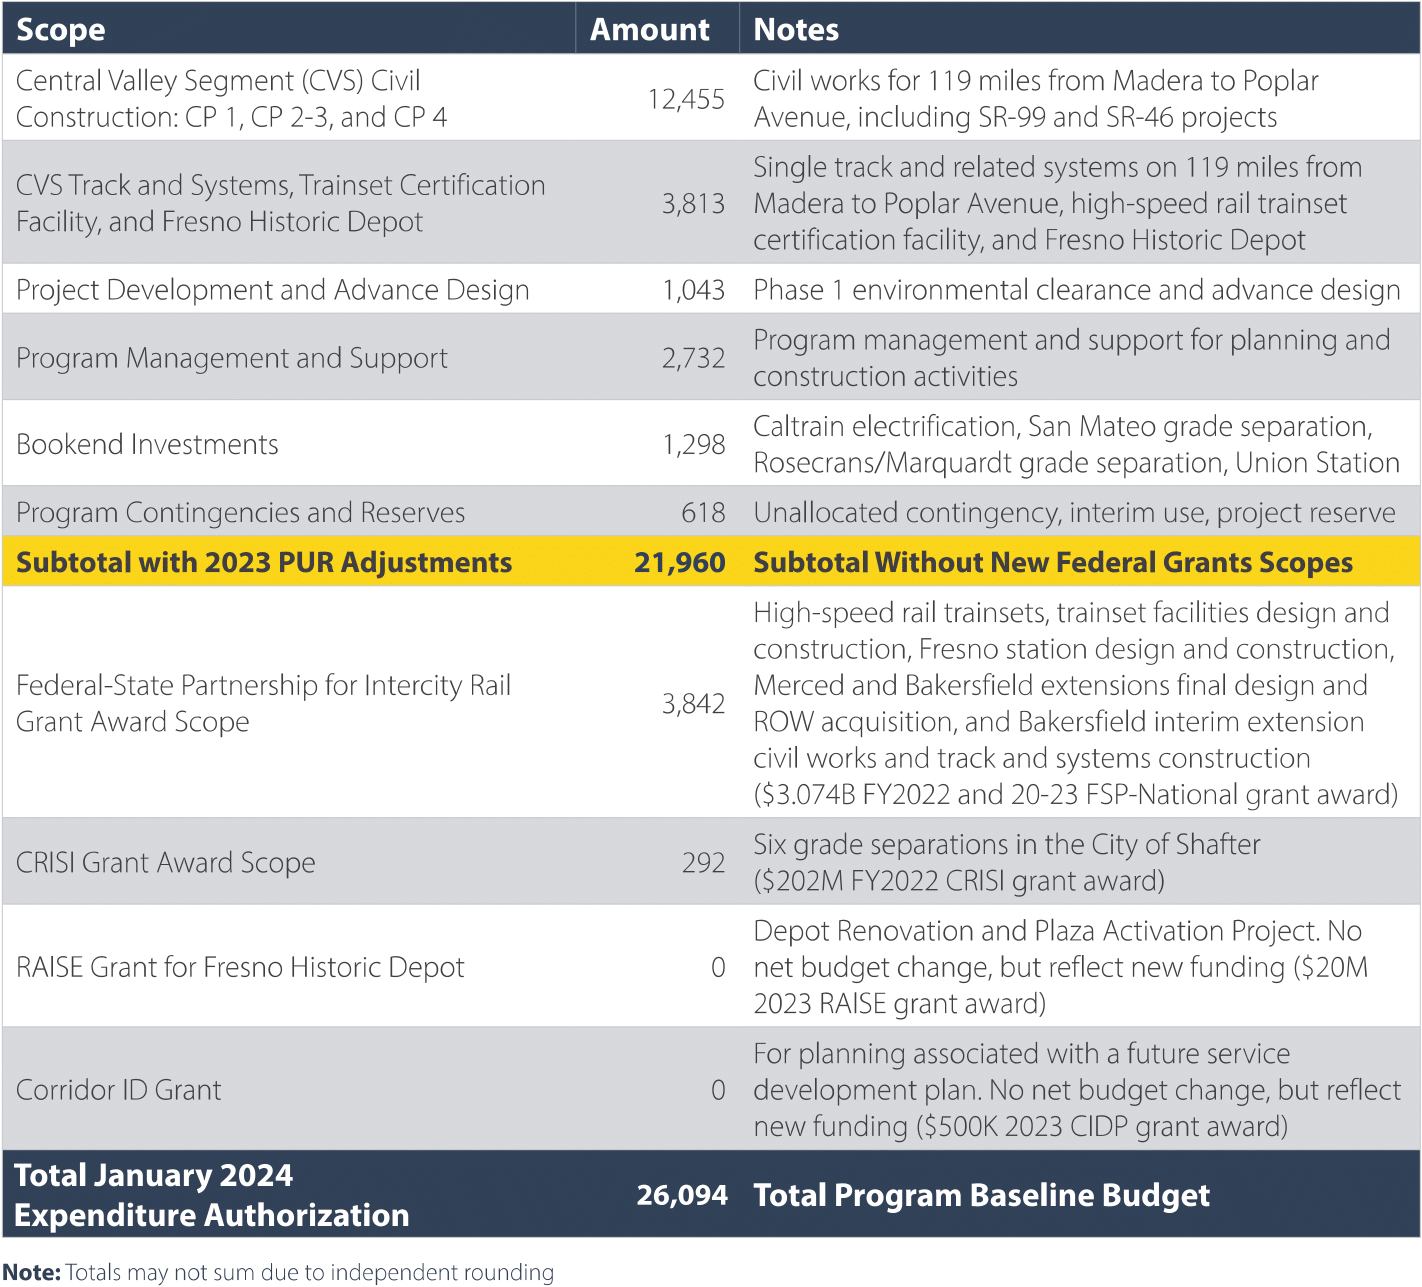
\includegraphics[width=\linewidth]{./attachments/budgeting}
\justifying

\section{Funding Sources}
\parindent20pt The project is funded through a combination of state, federal, and private investments. Key funding sources include: \begin{itemize}
	\item\textbf{Proposition 1A}: A \$9 billion grant for planning, construction, and administration \citep{proposition1A}
	\item Funds from the American Recovery and Reinvestment Act
	\item Federal-State partnership for Intercity Rail Grant Award
	\item CRISI Grant Award
	\item RAISE Grant for the Fresno Historic Depot
\end{itemize}

\centering\textbf{\underline{Figure 4.2: Authorized and Projected Future Funding \citep{ureport2025}}} \par
\noindent 
\vspace*{1em}
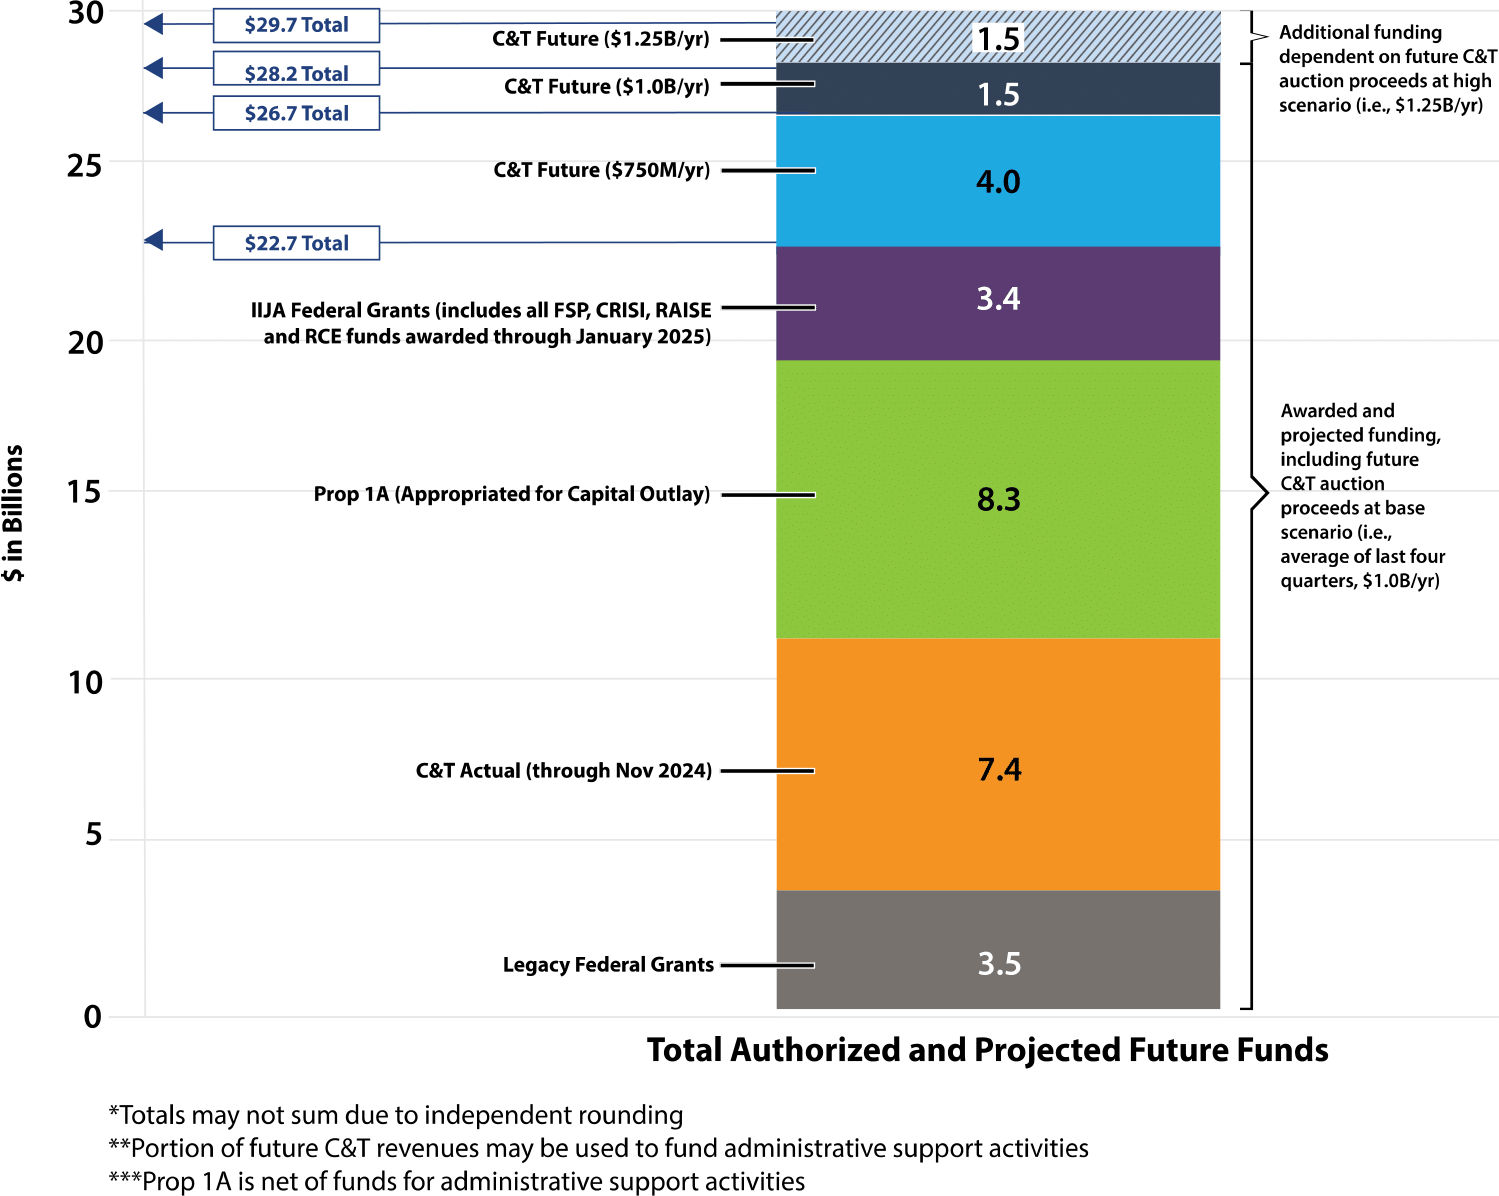
\includegraphics[width=\linewidth]{./attachments/fundalloc}
\justifying\par